\begin{frame}[fragile]{CNN - Normalization (Batch Norm)}
\begin{block}{What:}
    \begin{itemize}
        \item Normalize layer inputs over mini‑batch, then scale & shift.
    \end{itemize}
\end{block}

\begin{block}{Benefits:}
    \begin{itemize}
        \item Faster training,
        \item Allows higher learning rates,
        \item Reduces sensitivity to initialization,
        \item Acts as a regularizer.
    \end{itemize}
\end{block}

\begin{lstlisting}[language=Python, caption={Code snippet (PyTorch)}, basicstyle=\ttfamily\footnotesize]
import torch.nn as nn

bn = nn.BatchNorm2d(16)
x = bn(x)
\end{lstlisting}

\begin{block}{Note:}
    \begin{itemize}
        \item BatchNorm is typically used after convolutional layers and before activation functions.
        \item BatchNorm normalizes activations per‑batch, then scales/shifts them. 
    \end{itemize}
\end{block}
\end{frame}  

\begin{frame}{CNN - Normalization (Batch Norm)}
    \begin{figure}
    \centering
    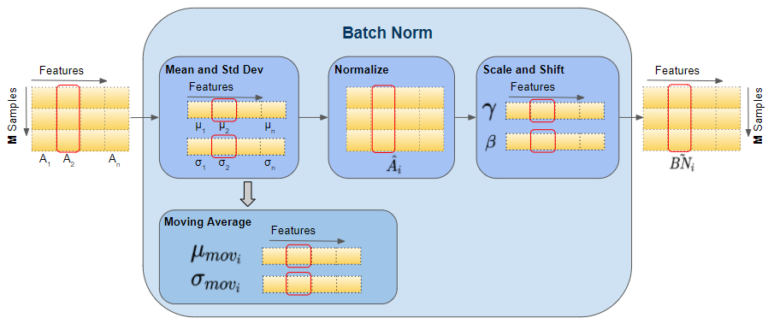
\includegraphics[width=0.95\textwidth,height=0.4\textheight,keepaspectratio]{images/batch-norm-unit.png}
    \end{figure}

    \begin{figure}
    \centering
    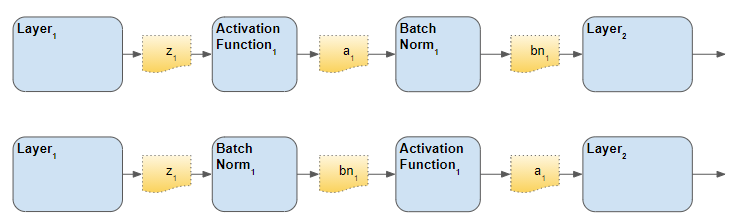
\includegraphics[width=0.95\textwidth,height=0.4\textheight,keepaspectratio]{images/batch-norm-sequence.png}
    \caption{Order of placement of Batch Norm layer}
    \end{figure}

    \href{https://towardsdatascience.com/batch-norm-explained-visually-how-it-works-and-why-neural-networks-need-it-b18919692739/}{More on Batch Norm from Towards Data Science}
\end{frame}